% Kolmogorov complexity against length, schematic.
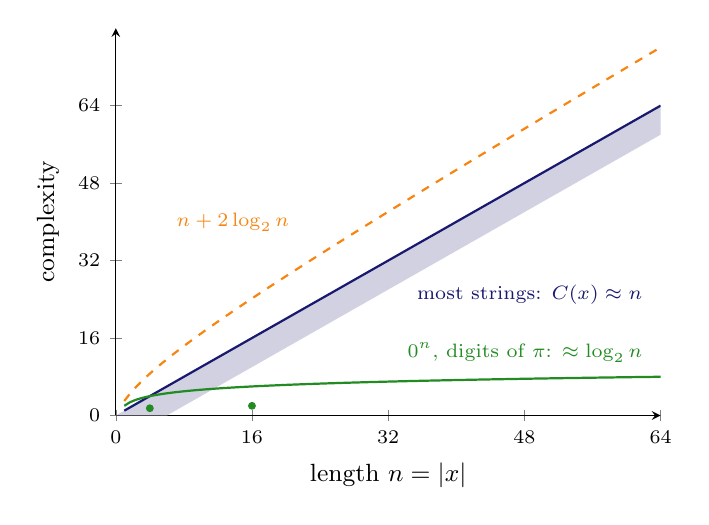
\begin{tikzpicture}
\begin{axis}[width=8.5cm,height=6.5cm,xmin=0,xmax=64,ymin=0,ymax=80,
  xlabel={length $n=|x|$},ylabel={complexity},xtick={0,16,32,48,64},ytick={0,16,32,48,64},
  axis lines=left,tick label style={font=\scriptsize},label style={font=\small}]
\addplot[fill=MidnightBlue!20,draw=none] coordinates {(0,0) (64,64) (64,58) (6,0)} --cycle;
\addplot[MidnightBlue,thick,domain=1:64,samples=60] {x};
\addplot[BurntOrange,dashed,thick,domain=1:64,samples=100] {x+2*ln(x+1)/ln(2)};
\addplot[ForestGreen,thick,domain=1:64,samples=100] {ln(x)/ln(2)+2};
\addplot[only marks,mark=*,mark size=1.2pt,ForestGreen] coordinates {(16,2) (4,1.5)};
\node[font=\scriptsize,MidnightBlue,anchor=east] at (axis cs:63,25) {most strings: $C(x)\approx n$};
\node[font=\scriptsize,BurntOrange,anchor=west] at (axis cs:6,40) {$n+2\log_2n$};
\node[font=\scriptsize,ForestGreen,anchor=south east] at (axis cs:63,9) {$0^n$, digits of $\pi$: $\approx\log_2n$};
\end{axis}
\end{tikzpicture}
